\chapter{序論}
\label{chap_Introduction}

XXXXXXXXXXXXXXXXX序論
%\begin{figure} % 特に強い理由がない限り、[htbp]のような指定はしないでください。
%  \centering
%  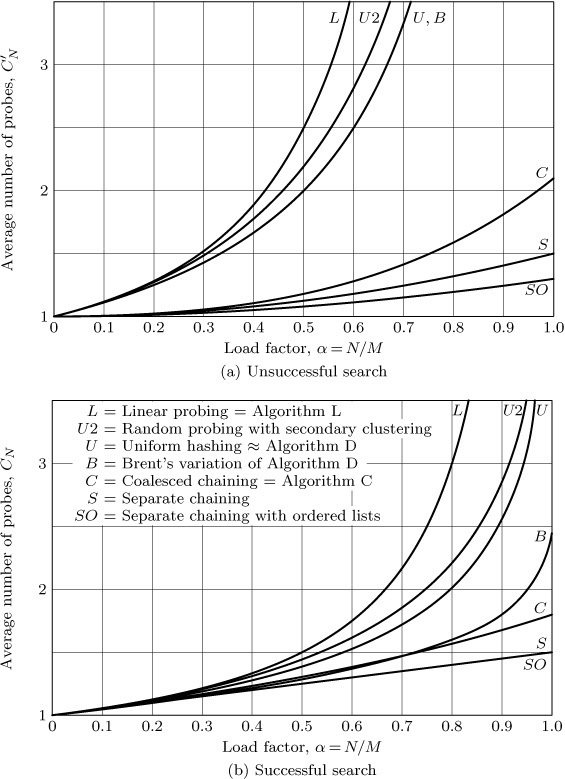
\includegraphics[width=10cm]{./figs/taocp_v3_fig44.png}
%  \caption{
%    Comparison of collision resolution methods: limiting values of the average number of probes as $M \rightarrow \infty$ \citep{knuth1998}.
%  }
%  \label{fig_taocp_v3_fig44}
%\end{figure}

%先行研究\footnote{脚注はこのように挿入します.}.

\section{先行研究}
現実的なハッシュテーブルを検討するには,
単にアルゴリズムのみならず,
対応する実実装との比較が望ましい.
ここでは,
実際に利用されているハッシュテーブルの実実装を示す.

\subsection{std::unorderd\_map}
C++ 標準のハッシュテーブル.
メモリ効率を重視しており速度は遅い.

\subsection{google::dense\_hash\_map}
最も探査の高速な実装の内の 1 つで,\cite{sparsehash2005}に含まれる.
スループットで 250 query/$\mu$s 程度
\footnote{AMD Ryzen7 1700 (8C/16T) 3.7 GHz の場合.詳細は,第\ref{chap_Results}章を参照.}
の探査速度を持つことから,
探査 1 回の実行時間は 4 ns
\footnote{
  $
    250{\rm [query \slash \mu s]}
    = \frac{1}{250} {\rm [\mu s \slash query]}
    = \frac{10^3}{250} {\rm [ns \slash query]}
    = 4 {\rm [ns \slash query]}
  $
}
である.このとき,3.7 GHz の CPU では単位 clock あたりの実行時間が,
$2.7 \times 10^{-1}$ [ns/clock]
\footnote{
  $
    \frac{1}{3.7 {\rm [GHz]}}
    = \frac{1}{3.7 \times 10^9}{\rm [sec]}
    = 2.7 \times 10^{-10}{\rm [sec]}
    = 2.7 \times 10^{-1}{\rm [ns/clock]}
  $
}
であるから,1 回の探査で消費する CPU cycle は
15 clock 程度
\footnote{
  $
    \frac{ 4 {\rm [ns/query]} }{ 2.7 \times 10^{-1} {\rm [ns/clock]} }
    = \frac{ 4 }{ 2.7 \times 10^{-1} } {\rm [clock/query]}
    \simeq 15 {\rm [clock/query]}
  $
}
である.

いくつかのハッシュテーブルでは,
key のハッシュ値をテーブルサイズに丸めるために剰余演算を用いる.
整数除算に必要な CPU cycle は 14--46 clocks 程度
\footnote{
  \cite{AgnerFog2018}より AMD Ryzen7 1700 の場合.
}
であるから,dense\_hash\_map の実行時間に対して計算量が大きい.
実際に,
dense\_hash\_map では,整数除算をしておらず,
ハッシュ値の LSB \footnote{Least Significant Bit の略記.最下位ビットのこと.} から
テーブルサイズ分の bit 数だけ bit mask 演算により取り出している.
これを実現するため,テーブルサイズは常に 2 のべき乗となるように制御されている.

また,メモリ使用量を削減するため,空マークを登録する必要があり,key として使用できない.
削除マークについても同様で,key とメモリを共有しているため,削除が必要な場合は,削除マークを登録する必要があり,key として使用できなくなる.

\subsection{ska::flat\_hash\_map}

Robin Hood hashing の実実装の内の一つ.
条件次第で dense\_hash\_map より探査が高速であることを謳う.
Robin Hood hashing は衝突解決法の一つで,
singly linked list を用いて,
より近い位置に要素が移動するように調整する.
実際の探査時は,Linear probing により要素を検索する.
Linear probing のコストに配慮し,
探査を $log_2(n)$ に制限している (ただし $n$ はテーブルサイズ) \cite{Skarupke2017}.


\begin{table}[hbtp]
  \caption{各実装の比較.}
  \begin{tabular}{ccccc} \hline
    Implementation of hash table & Algorism              & Successful lookup & Unsuccessful lookup & Memory efficiency \\ \hline
    std::unorderd\_map           & Open hashing $^{a)}$   & bad               & bad                 & good              \\ 
    google::dense\_hash\_map     & Closed hashing $^{b)}$ & good              & good                & medium            \\
    ska::flat\_hash\_map         & Closed hashing $^{c)}$ & good              & good                & bad               \\ \hline
  \end{tabular}
  \\ 
  $^{a)}$ Chaining, 
  $^{b)}$ Quadratic probing,
  $^{c)}$ Robin Hood hashing (One of the linear probing)
  \\
  \label{table_env}
\end{table}


%\begin{threeparttable}[hbtp]
%  \caption{各実装の比較.\vspace{-2.5mm}}
%  \begin{tabular}[]{cccc}\hline
%     Implementation of hash table & Algorism & Successful lookup & Unsuccessful lookup \rule[0pt]{0pt}{0pt} \\ \hline
%    std::unorderd\_map & Open hashing \tnote{Chaining} & bad & \rule[0pt]{0pt}{0pt} \\ 
%    google::dense\_hash\_map & Closed hashing \tnote{Quadratic probing} & good& \\
%    ska::flat\_hash\_map & Closed hashing \tnote{Robin Hood hashing (One of the linear probing)} & good & \\ \hline
%  \end{tabular}
%  \begin{tablenotes}[para] %(default:normal) % para,flushleft,online,normal
%  \item[1] ......
%  \item[2] ......
%  \end{tablenotes}
%  \label{table_hashT_imp}
%\end{threeparttable}
%\vspace{2.5mm}
%あああああああああああ

%\begin{table}[hbtp]
%  \begin{center}
%    \caption{各実装の比較.}
%    \begin{tabular}{cccc} \hline
%      Implementation of hash table & Algorism & Successful lookup & Unsuccessful lookup \rule[0pt]{0pt}{0pt} \\ \hline
%      std::unorderd\_map & Open hashing / & bad & \rule[0pt]{0pt}{0pt} \\ 
%                         & Chaining &  & \rule[0pt]{0pt}{0pt} \\ 
%      google::dense\_hash\_map & Closed hashing / & good& \\
%                               & Quadratic probing & & \\
%      ska::flat\_hash\_map & Closed hashing / & good & \\
%                           & Robin Hood hashing & & \\
%                           & (One of the linear probing) & & \\ \hline
%    \end{tabular}
%  \end{center}
%  \label{table_env}
%\end{table}

%\begin{table}[hbtp]
%  \begin{center}
%    \caption{各実装の比較.}
%    \begin{tabular}{cccc} \hline
%      Implementation of hash table & std::unorderd\_map & google::dense\_hash\_map & ska::flat\_hash\_map \rule[0pt]{0pt}{0pt} \\ \hline
%      Algorism & Open hashing / & Closed hashing        & Closed hashing \\
%               & Chaining       & Quadratic probing     & Robin Hood hashing \\
%               &                &                       & (One of the linear probing) \\
%        Successful lookup & bad & good & good \\
%      Unsuccessful lookup & bad & good & good \\ \hline
%    \end{tabular}
%  \end{center}
%  \label{table_env}
%\end{table}

\section{Purpose}
研究目的.



















